\documentclass[times, utf8, zavrsni]{fer}
\usepackage{booktabs}
\usepackage{natbib}
\usepackage{biblatex}
\addbibresource{literatura.bib}
\addto\captionscroatian{\renewcommand{\bibname}{Literatura}} % Promjena naslova na literatura

\begin{document}

\thesisnumber{1017}

\title{Sustav za praćenje vremenske prognoze}

\author{Kristo Palić}

%\maketitle

\zahvala

\tableofcontents

\chapter{Uvod}
Vremenska prognoza ima ključnu ulogu u našim svakodnevnim životima, utjeće na odluke koje se kreću od odabira odjeće do planiranja putovanja. Preciznost i dostupnost vremenske prognoze postala je sve važnija s rastućim utjecajem klimatskih promjena. Stoga, postoji potreba za pouzdanim i pristupačnim sustavima za praćenje vremenske prognoze. Završni rad fokusira se na oblikovanje i izgradnju takvog sustava. Cilj je razviti korisničko sučelje koje će na čitljiv i interaktivan način prikazivati podatke o vremenskoj prognozi. Podatke će dohvaćati putem aplikacijskog programskog sučelja WeatherAPI \cite{weather_API} \textit{(engl. API - Application Programming Interface)} što omogućava pružanje ažuriranih informacija u stvarnom vremenu. Osim prikaza trenutne vremenske prognoze za korisnikovu lokaciju, sustav će omogućiti pretraživanje drugih lokacija te pružiti predviđanje vremenske prognoze za odabrane lokacije. Ova funkcionalnost omogućava korisnicima da planiraju događaje u skladu s očekivanim vremenskim uvjetima. Kroz ovaj rad demonstrirat će se proces oblikovanja i izgradnje ovog sustava, kao i razmatranje mogućih izazova i rješenja pronađenih tijekom njegove izrade. Pravovremene obavijesti o vremenskim uvjetima i mogućim nepogodama iznimno su bitne za prevenciju štete i zaštitu života. S obzirom na promjenjivost klime, nepogode postaju sve češća pojava, donoseći sa sobom značajnu godišnju štetu. Materijalna šteta izazvana nepogodama uključuje uništenje infrastrukture, poljoprivrednih kultura te stambenih i poslovnih objekata. No, štetu ne treba gledati samo kroz prizmu materijalnog - nematerijalna šteta, koja obuhvaća emocionalni stres i utjecaj na mentalno zdravlje, može biti jednako devastirajuća, ako ne i više u slučaju gubitka ljudskih života. Utjecaj klimatskih promjena na vremenske uvjete sve je vidljiviji. Ekstremni vremenski uvjeti kao što su snažne oluje, poplave, suše i toplinski valovi postaju sve češći. S obzirom na ovu problematiku, precizna i ažurirana vremenska prognoza više nije samo alat za svakodnevno planiranje, već neophodan resurs za pravovremeno reagiranje na nadolazeće promjene. Praćenje količine padalina jedan je od ključnih faktora za održavanje sigurnosti i funkcionalnosti gradskih usluga. Nagli porast količine padalina može ukazivati na potencijalnu prijetnju od poplava. Pravovremeno upozorenje gradskih službi o mogućnosti poplava može omogućiti pravovremene mjere zaštite i smanjivanje rizika. Na taj način, sustav za praćenje vremenskih uvjeta postaje ključan element zaštite građana i imovine. U svrhu navedenog, predloženi sustav za praćenje vremenske prognoze osmišljen je da na čitljiv, brz i efikasan način dostavi korisnicima potrebne informacije. Kroz daljnje poglavlje, predstavit će se detalji vezani za dizajn i implementaciju ovog sustava, s posebnim fokusom na korisničko sučelje, dostupnost podataka te pouzdanost i točnost vremenskih prognoza.


\chapter{Arhitektura i dizajn sustava}
Arhitektura aplikacije sastoji se od klijentske aplikacije, web poslužitelja i baze podataka te predstavlja ključni dio proizvoda. Ovaj tip arhitekture omogućuje razdvajanje odgovornosti na tri glavna dijela sustava što pomaže u poboljšanju performansi, skalabilnosti i sigurnosti aplikacije. Osim navedenog, aplikacija koristi aplikacijsko programsko sučelje WeatherAPI pomoću kojeg dohvaća redovno ažurirane podatke o trenutnom vremenu i vremenskoj prognozi. Poslužitelj-klijent arhitektura je model dizajna u kojem poslužitelj pruža resurse ili usluge, a klijent ih koristi. Povijesno gledano, ovaj model arhitekture postao je popularan s rastom distribuiranih sistema, uključujući razvoj internetskih aplikacija. Značajke poslužitelj-klijent arhitekture uključuju:
\begin{itemize}
    \item \textbf{asimetričnost}: poslužitelj i klijent imaju različite uloge.
    \item \textbf{modularnost}: klijent i poslužitelj mogu se razvijati neovisno.
    \item \textbf{skalabilnost}: dodavanje klijenata ne bi trebalo utjecati na performanse poslužitelja.
\end{itemize}
Prednosti ovog modela uključuju:
\begin{itemize}
    \item \textbf{efikasnost}: podaci se obrađuju na poslužitelju, tako da klijenti mogu biti manje zahtjevni.
    \item \textbf{fleksibilnost}: moguće je koristiti različite vrste klijenata s istim poslužiteljem.
\end{itemize}
Međutim, ovaj model ima mane: mogućnost preopterećenja poslužitelja i potencijalne probleme sa sigurnošću, budući da poslužitelj predstavlja centraliziranu točku napada. REST (Representational State Transfer) je arhitekturni stil koji je postao vrlo popularan za dizajniranje mrežnih aplikacija. REST osigurava jednostavnost i skalabilnost putem operacija "bez stanja" (engl. stateless), što znači da se svaki zahtjev može obraditi neovisno o prethodnim zahtjevima. Osim toga, REST koristi standardne HTTP metode, što olakšava implementaciju. U poslužitelj-klijent arhitekturi, odgovornosti su jasno podijeljene između klijenta, poslužitelja i baze podataka. Klijent je odgovoran za slanje zahtjeva poslužitelju i prikaz podataka korisniku. Poslužitelj je odgovoran za obradu zahtjeva, pristupanje podacima iz baze podataka i slanje odgovora klijentu. Baza podataka je odgovorna za pohranu, dohvat i ažuriranje podataka. U kontekstu naše aplikacije, klijent (web aplikacija) prikazuje podatke o vremenskoj prognozi korisniku, a poslužitelj koristi WeatherAPI za dohvat tih podataka. Baza podataka koristi se za pohranu korisničkih postavki i pretraživanja, pružajući personalizirano iskustvo. Ovaj dizajn omogućava efikasnu obradu zahtjeva i skalabilnost aplikacije.

\section{Opća arhitektura sustava}

Sustav je projektiran kao klijent-poslužitelj aplikacija. Klijentska strana, koja se pokreće u korisnikovom web pregledniku, razvijena je koristeći React Typescript \cite{typescript-react}. Klijent komunicira s poslužiteljem putem HTTP zahtjeva za dohvat vremenskih podataka. Poslužiteljska strana, razvijena u Pythonu, služi kao posrednik između klijenta i aplikacijskog programskog sučelja WeatherAPI. Kada poslužitelj primi zahtjev od klijenta, šalje zahtjev sučelju, obrađuje odgovor i šalje podatke natrag klijentu.

\section{Dizajn korisničkog sučelja}
Dizajn korisničkog sučelja temelji se na nekoliko ključnih principa. Prvi je konzistentnost, koja osigurava da se slične komponente korisničkog sučelja konzistentno ponašaju i izgledaju. Drugi je feedback, gdje korisničko sučelje pruža jasne povratne informacije korisniku o rezultatu njegovih akcija. Također, tu je i princip minimalizma, koji naglašava kako sučelje treba biti jednostavno s manje opcija i funkcionalnosti kako bi se izbjegla konfuzija. Česte greške u dizajnu korisničkog sučelja uključuju:
\begin{itemize}
    \item \textbf{pretrpanost informacijama}
    \item \textbf{nedostatak povratnih informacija korisniku}
    \item \textbf{narušavanje konzistentnosti}
    \item \textbf{nedostatak intuitivnosti}
\end{itemize}
U našem dizajnu nastojali smo izbjeći ovakve pogreške pružanjem jednostavnog i intuitivnog sučelja. Intuitivnost u dizajnu postignuta je kroz upotrebu poznatih simbola i stilskih uzoraka, što korisnicima omogućuje da lako shvate kako komunicirati s korisničkim sučeljem. Na primjer, koristimo ikonu povećala za opciju pretrage, što je opće prihvaćen simbol za pretragu. Prikaz vremenske prognoze za određeni dan sadrži datum, ikonu i dvije brojke koje označavaju maksimalnu i minimalnu temperaturu toga dana. Takav prikaz nije potrebno posebno opisivati jer je intuitivno da govorimo o dnevnoj vremenskoj prognozi za određeni grad. Odabrani dan veće je dimenzije od ostalih ponuđenih dana i samim time korisnik na intuitivan način zna koji je dan odabran bez potrebe za detaljnijim objašnjenjem. Nadalje, tako odabrani dan imati će prikaz vlastite vremenske prognoze po satima. Vremenska prognoza po satima sadrži sat u danu čiju prognozu predstavlja, sliku koja opisuje kakvo će vrijeme biti, postotak vjerojatnosti padalina u tom satu, jačinu i smjer vjetra u kilometrima na sat. Glavni zaslon korisničkog sučelja pruža trenutnu vremensku prognozu za korisnikovu lokaciju, što omogućava korisnicima da odmah vide najvažnije informacije. Osim toga, korisnici mogu unijeti ime drugog grada u pretraživačku traku za prikaz vremenske prognoze nove lokacije, pružajući lakoću upotrebe i fleksibilnost u pružanju informacija. Korisničko sučelje osmišljeno je s ciljem jednostavnosti i čitljivosti.

\section{Komunikacija s WeatherAPI-jem}

Komunikacija sa aplikacijskim programskim sučeljem WeatherAPI ostvarena je kroz HTTP GET/POST zahtjeve. Zahtjevi su poslani s poslužiteljske strane koristeći Pythonov requests modul. Odgovori od API-ja obrađeni su i proslijeđeni klijentskoj strani u obliku JSON odgovora. HTTP \textit{(engl. HyperText Transfer Protocol)} je temeljni protokol za prijenos podataka na internetu. Koristi se za slanje zahtjeva od klijenta prema poslužitelju i za prenos odgovora od poslužitelja prema klijentu. HTTP podržava različite metode zahtjeva, uključujući GET, POST, PUT, DELETE. Ove metode omogućuju klijentu da obavi različite operacije, kao što su dohvat podataka (GET), slanje podataka (POST), ažuriranje podataka (PUT) ili brisanje podataka (DELETE). HTTP je razvijen 1991. godine i do danas je postao standard za web komunikaciju. Struktura HTTP zahtjeva sastoji se od metode zahtjeva, zaglavlja koje sadrže metapodatke i tijela zahtjeva koje može sadržavati podatke. U kontekstu naše aplikacije, koristimo HTTP GET zahtjeve za dohvat podataka o vremenskoj prognozi od WeatherAPI-ja i HTTP POST zahtjeve za slanje podataka, poput korisničkih postavki. JSON (JavaScript Object Notation) je format za razmjenu podataka koji se često koristi u web aplikacijama. Jednostavan je za čitanje i pisanje, a podržan je u većini modernih programskih jezika, uključujući Python. JSON objekt se sastoji od parova ključ-vrijednost, što omogućava lako mapiranje na objekte u programskim jezicima. U našoj aplikaciji, odgovori od WeatherAPI-ja obrađeni su i proslijeđeni klijentskoj strani u obliku JSON odgovora. Ovo omogućava lako korištenje i manipulaciju podacima na klijentskoj strani.

\section{Upravljanje bazom podataka}

Baza podataka temeljni je dio našeg sustava, a za njeno upravljanje koristimo PostgreSQL, moćan otvoreni sustav za upravljanje bazama podataka koji pruža robusnost, skalabilnost i visoke performanse. PostgreSQL ima mnogo prednosti koje ga čine idealnim za naš sustav. Prvo, podržava velik broj tipova podataka, što omogućava fleksibilnost u modeliranju naših podataka. Drugo, ima snažne mogućnosti za transakcijsko upravljanje, što omogućava sigurno i pouzdano upravljanje podacima. Treće, njegove mogućnosti skaliranja omogućuju nam da lako rukujemo velikom količinom podataka. Unatoč tome što je iznimno snažan, ima neke nedostatke. Prvo, može biti složen za konfiguriranje i optimizirati, osobito za velike sustave. Drugo, iako podržava veliki broj funkcionalnosti, neke od naprednijih značajki mogu biti teške za upotrebu bez dubljeg razumijevanja. Za upravljanje našom PostgreSQL bazom podataka koristimo PgAdmin4, popularan alat za upravljanje PostgreSQL bazama podataka. PgAdmin4 pruža grafičko sučelje koje omogućava lako upravljanje, praćenje i optimizaciju baze podataka. Također, podržava izvođenje složenih SQL upita, što omogućava fleksibilno upravljanje podacima. Iako PgAdmin4 pruža mnoge mogućnosti, njegovo sučelje može biti teško za upotrebu za one koji nisu upoznati s SQL-om ili administracijom baza podataka. U našem sustavu, koristimo bazu podataka za spremanje podataka o korisnicima. Kada korisnik prvi put pristupi sustavu, generira se token koji se koristi za identifikaciju korisnika pri kasnijim pristupima uslugama aplikacije. Navedena arhitektura omogućuje nam da osiguramo sigurnost i privatnost korisničkih podataka, dok istovremeno pružamo personalizirano korisničko iskustvo.

\section{Sigurnost i zaštita podataka}

S obzirom na prirodu podataka koje sustav obrađuje, implementirane su osnovne mjere zaštite podataka. Svi podaci preneseni između klijenta, poslužitelja i API-ja šifrirani su koristeći HTTPS protokol. Dodatno, baza podataka zaštićena je od SQL injekcija korištenjem parametriziranih upita. Sigurnost i zaštita podataka od vitalne su važnosti u svakoj aplikaciji. U našem sustavu podatci se prenose između klijenta, poslužitelja i API-ja koristeći HTTPS protokol. HTTPS je sigurna verzija HTTP protokola koja koristi SSL/TLS protokole kako bi osigurala enkriptiranu komunikaciju i siguran prijenos podataka. SQL injekcija je vrsta napada na sigurnost u kojem napadač ubacuje zlonamjerne SQL naredbe u upit. To se obično postiže putem ulaznih polja koja nisu dovoljno zaštićena. Kako bi zaštitili našu bazu podataka od SQL injekcija, koristimo parametrizirane upite. Parametrizirani upiti osiguravaju da ulazni podaci budu tretirani isključivo kao vrijednosti, a ne kao dio SQL naredbe. Kada je u pitanju pohrana lozinki korisnika, koristimo strategiju "sol i papar" \textit{(engl. salt and pepper)} za dodatnu sigurnost. "Salt" je slučajni niz koji se dodaje originalnoj lozinci prije njenog hashiranja, dok je "pepper" tajni niz dodan lozinci nakon "soljenja". Ova dva koraka zajedno čine lozinku mnogo težom za dešifriranje čak i ako napadač dobije pristup hashiranim lozinkama. Međutim, uvijek postoji rizik od napada pa je važno kontinuirano nadograđivati i poboljšavati naše sigurnosne mjere. Povijesno, jedna od najvećih prijetnji na internetu su DDoS napadi \textit{(engl. Distributed Denial of Service)}, gdje napadač preplavi mrežni resurs s toliko zahtjeva da postaje nedostupan. Kako bismo se zaštitili od ovakvih napada, mogli bismo implementirati razne tehnike za ublažavanje DDoS-a, kao što su ograničavanje broja zahtjeva po IP adresi ili korištenje CDN-a \textit{(engl. Content Delivery Network)} koji može apsorbirati veliki broj zahtjeva.

\chapter{Implementacija}
\section{Izgradnja klijentske aplikacije}

Klijentska aplikacija izgrađena je koristeći React Typescript, s fokusom na modularnost i održivost. Cjelokupna aplikacija organizirana je oko centralne App.tsx komponente koja upravlja rutama i navigacijom između različitih stranica. React Typescript kombinira moć Reacta, biblioteke za izgradnju korisničkih sučelja, s robusnošću Typescripta, nadograđenog JavaScripta s dodatkom statičkih tipova. Korištenjem React Typescripta za izgradnju klijentske aplikacije, možemo profitirati od modularnosti, efikasnosti i održivosti koje ove tehnologije nude. Struktura koda naše aplikacije je organizirana i modulirana. Kôd je podijeljen u manje, samostalne komponente koje su odgovorne za specifične dijelove korisničkog sučelja. Ova struktura omogućava lakše održavanje i ažuriranje koda, kao i veću ponovnu upotrebljivost komponenti. Naše smjernice za kodiranje slijede vanjske standarde kao što su AirBnB Style Guide za React i TypeScript. Ove smjernice pomažu nam da održimo kôd čistim, konzistentnim i lako čitljivim. Primjerice, svaka komponenta ima svoju datoteku, koristimo funkcionalne komponente gdje god je to moguće, a Hooks koristimo za upravljanje stanjima i životnim ciklusima komponenti. Koristimo React Router za dinamičko upravljanje putanjama na klijentskoj strani, što omogućava korisnicima fluidno i intuitivno iskustvo pregledavanja, bez nepotrebnog učitavanja stranica. Koristeći React Typescript, uspjeli smo izgraditi klijentsku aplikaciju koja je skalabilna, održiva i koja pruža vrhunsko korisničko iskustvo. React Router je biblioteka za upravljanje putanjama \textit{(engl. routing)} koja se koristi u React aplikacijama. Omogućuje navigaciju među različitim komponentama u aplikaciji bez potrebe za osvježavanjem stranice. React Router koristi koncept dinamičkog usmjeravanja \textit{(engl. dynamic routing)}, što znači da se komponente za određene rute prikazuju samo kada je ruta aktivna. Ovo pomaže pri optimizaciji performansi aplikacije. Jedna od ključnih komponenti React Routera je BrowserRouter, koja koristi HTML5 povijest API-a (pushState, replaceState i popstate događaj) za održavanje korisničke UI-a u sinkronizaciji s URL-om. Unutar BrowserRouter komponente, koristimo Route komponentu kako bismo definirali različite rute u našoj aplikaciji. Svaka Route komponenta mapira putanju URL-a na određenu komponentu koja se treba generirati kada je ta putanja aktivna. Evo primjera kako to izgleda u kodu:

\begin{verbatim}
<BrowserRouter>
  <div>
    <Route exact path="/" component={Home} />
    <Route path="/about" component={About} />
    <Route path="/contact" component={Contact} />
  </div>
</BrowserRouter>
\end{verbatim}
U ovom primjeru, kada korisnik posjeti osnovnu putanju (`/`), generira se komponenta `Home`. Ako korisnik posjeti `/about`, generira se komponenta `About`, i slično. `Link` komponenta se koristi za kreiranje navigacijskih veza u aplikaciji. Klik na `Link` komponentu ažurira URL i generira novu komponentu bez osvježavanja stranice. Primjer za to bi izgledao ovako:

\begin{verbatim}
<div>
  <Link to="/">Home</Link>
  <Link to="/about">About</Link>
  <Link to="/contact">Contact</Link>
</div>
\end{verbatim}
Osim toga, React Router nudi brojne druge značajke kao što su `Switch` (za generiranje samo prve `Route` ili `Redirect` koja se podudara s lokacijom), `Redirect` (za preusmjeravanje na drugu rutu), `withRouter` (za pristup povijesti, lokaciji i podudaranju izvan usmjeravajuće komponente). React Router je ključan alat za svaku aplikaciju aplikaciju podijeljenu na komponente, gdje je u svakom trenutku samo jedna stranica (komponenta) aktivna\textit{(engl. single-page application)} izrađenu s Reactom, omogućujući kompleksne scenarije usmjeravanja uz minimalan napor.
.
\newpage
\subsection{Struktura koda}

Glavna struktura koda organizirana je na sljedeći način:

\begin{itemize}
    \item \textbf{App.tsx} je glavna komponenta aplikacije. Uključuje preusmjeravanje do različitih stranica i kontrolu pristupa ovisno o tome je li korisnik prijavljen ili nije.
    \item \textbf{models} direktorij sadrži modele koji se koriste za automatsko spremanje podataka s poslužitelja.
    \item \textbf{pages} sadrži sve stranice koje su dostupne u aplikaciji. Svaka stranica je smještena u vlastiti direktorij i sastoji se od Typescript datoteke i pripadne joj CSS datoteke.
    \item \textbf{components} direktorij sadrži  komponente koje su dio svake stranice, kao što su zaglavlje \textit{(engl. header)} i podnožje \textit{(engl. footer)}.
\end{itemize}

\subsection{Glavna komponenta}

Glavna komponenta, poznata kao `App.tsx` u React Typescript aplikacijama, ključna je za upravljanje strukturom aplikacije. Ova komponenta često djeluje kao "okvir" za sve ostale komponente unutar aplikacije. Zbog svoje važnosti, posebna pozornost mora biti usmjerena prema njenoj strukturi i funkcionalnostima koje nudi. App.tsx komponenta u ovoj aplikaciji koristi `react-router-dom` \cite{reactrouter} biblioteku kako bi upravljala rutama i navigacijom kroz cijelu aplikaciju. Na temelju trenutne rute u URL-u, ova komponenta određuje koja druga komponenta treba biti generirana. S obzirom na dinamičku prirodu ovog tipa usmjeravanja, moguće je generirati bilo koju komponentu u bilo kojem trenutku, što pridonosi fleksibilnosti i korisničkom iskustvu. Ovaj odlomak koda definira različite rute unutar aplikacije. Svaka ruta asocirana je s određenom komponentom koja se prikazuje kada je ta ruta aktivna.
\begin{verbatim}
<Routes>
  <Route path="/" element={<Homepage />} /> 
  <Route path="/weather" element={<Weather />} /> 
  <Route path="/login" element={<Login />} /> 
  <Route path="/register" element={<Register />} /> 
</Routes>

\end{verbatim}
Osim upravljanja rutama i navigacijom, `App.tsx` komponenta u ovoj aplikaciji ima ključnu ulogu u autentikaciji korisnika. Prilikom pokretanja aplikacije, provjerava se postoji li pristupni token \textit{(engl. access token)} u korisnikovoj sesiji. Pristupni token je informacija koja se pohranjuje u sesiji kada se korisnik prijavi i koristi se za provjeru korisnikovih prava prilikom pristupa različitim dijelovima aplikacije. Na temelju dostupnosti ovog tokena, `App.tsx` odlučuje prikazati standardno zaglavlje aplikacije ili zaglavlje koje je prilagođeno za prijavljene korisnike. Ovo omogućuje da aplikacija pruži personalizirano korisničko iskustvo, pružajući različite opcije i funkcionalnosti ovisno o tome je li korisnik prijavljen ili ne. Svaka ruta kojom `App.tsx` upravlja asocirana je s određenom komponentom. Kada je ruta aktivna, odgovarajuća komponenta se prikazuje. Ovo omogućuje jednostavnu navigaciju između različitih dijelova aplikacije, s komponentama koje su izolirane i neovisne jedna o drugoj. Takva modularnost olakšava razvoj, testiranje i održavanje aplikacije, jer svaka komponenta može biti razvijena i održavana zasebno. Ukratko, glavna `App.tsx` komponenta igra ključnu ulogu u upravljanju putanjama, navigacijom i autentikacijom unutar aplikacije, osiguravajući da se korisnicima pruži fleksibilno, sigurno i ugodno korisničko iskustvo.

\subsection{Axios}
Kao što je već spomenuto, sustav koristi biblioteku Axios za postavljanje HTTP zahtjeva. Axios je vrlo popularna biblioteka JavaScripta za izvršavanje HTTP zahtjeva. Nudi sučelje visoke razine koje omogućuje lako izvršavanje zahtjeva s obećanjima, tj. asinkronim operacijama koje omogućuju obradu HTTP odgovora kad god su dostupni, bez blokiranja ostatka koda. Jedna od ključnih prednosti Axiosa je mogućnost stvaranja "instance" Axiosa. Instance omogućuju predefiniranje konfiguracije za specifične potrebe aplikacije. U ovom slučaju, stvorena je instanca Axiosa sa predefiniranom osnovnom URL adresom, što znači da se svaki zahtjev poslan kroz tu instancu automatski usmjerava na taj URL. To olakšava organizaciju koda i poboljšava njegovu čitljivost. Primjer navedenog u kodu:
\begin{verbatim}
import axios from 'axios'

export const AxiosInstance = axios.create({ 
    baseURL: 'http://localhost:5000/'
})
\end{verbatim}
Osim toga, moguće je dodati presretače (engl. interceptors) zahtjeva ili odgovora koji mogu mijenjati zahtjeve ili odgovore prije nego što su poslani na poslužitelj ili prije nego što ih se obradi na klijentskoj strani. U ovom slučaju, interceptor zahtjeva dodan je Axios instanci kako bi se u svaki zahtjev dodalo zaglavlje 'Authorization' s pristupnim tokenom iz sesije korisnika. Ako pristupni token ne postoji, ali postoji osvježavajući token, tada se pristupni token osvježava pomoću zahtjeva na poseban krajnji URL. Ovdje je prikazano kako smo to implementirali:

\begin{verbatim}
AxiosInstance.interceptors.request.use(async request => {
    let token = sessionStorage.getItem('accessToken')
    let refreshToken = sessionStorage.getItem('refreshToken')
    if (token && request.headers) {
        request.headers['Authorization'] = 'Bearer ' + token
    } else if (refreshToken) {
        const response = await axios.post
            ('http://localhost:5000/refresh', 
             { token: refreshToken })
        let newToken = response.data.access_token
        sessionStorage.setItem('token', newToken)
        request.headers['Authorization'] = 'Bearer ' + token
    }
    return request
})
\end{verbatim}
Dakle, Axios pruža snažan alat za postavljanje HTTP zahtjeva, nudeći visoku modularnost i prilagodljivost koje su ključne za razvoj moderne web aplikacije.

\subsection{Automatizirana obrada podataka}
U suvremenom razvoju softvera, automatizacija obrade podataka ključna je za povećanje učinkovitosti i smanjenje mogućnosti pogrešaka koje mogu nastati prilikom ručne obrade. U kontekstu klijentske aplikacije, automatizirana obrada podataka ostvarena je kroz modeliranje podataka koje vraća poslužitelj. U usporedbi s tradicionalnom, ručnom obradom podataka, automatizirana obrada podataka pruža brojne prednosti. Prvo, smanjuje količinu potrebnog koda, što olakšava održavanje i nadogradnju aplikacije. Drugo, smanjuje se mogućnost pogrešaka koje mogu nastati prilikom ručne obrade podataka. Treće, automatizirana obrada podataka poboljšava čitljivost koda i modularnost, što olakšava razumijevanje koda i njegovu ponovnu upotrebu. Međutim, primjena automatizirane obrade podataka može imati i početne poteškoće, pogotovo kada se suočavamo sa složenim i detaljnim strukturama podataka. U takvim slučajevima, potrebno je pažljivo dizajnirati modele podataka kako bi odgovarali strukturama podataka koje vraća poslužitelj. Na primjer, u klijentskoj aplikaciji implementiran je model "Astronomy" koji odgovara strukturi podataka koju vraća WeatherAPI za astronomske informacije. Ovaj model precizno mapira podatke u strukturu koja je jednostavna za obradu unutar aplikacije. Automatizirana obrada podataka unutar klijentske aplikacije omogućava brzu i efikasnu obradu velikih količina podataka, dok se održava čitljivost i modularnost koda. Bez obzira na početne poteškoće, ova metoda obrade podataka ima ključnu ulogu u stvaranju učinkovite i održive aplikacije. Direktorij "models" ima ključnu ulogu u obradi podataka koje klijentska aplikacija prima od poslužitelja. Svaka datoteka unutar ovog direktorija predstavlja model koji odgovara strukturi podataka koju poslužitelju vraća sučelje WeatherAPI za određene vremenske uvjete. Modeli su oblikovani tako da točno odgovaraju strukturi JSON odgovora koji se dobiva od poslužitelja. To omogućava aplikaciji da automatski mapira podatke u modele bez potrebe za ručnom obradom. Ovdje je prikazan kod za model "Astronomy":

\begin{verbatim}
export type Astronomy = {
    is_moon_up:number
    is_sun_up:number
    moon_illumination:string
    moon_phase:string
    moonrise:string
    moonset:string
    sunrise:string
    sunset:string
}
\end{verbatim}
Tako dobivenim informacijama možemo lako i učinkovito manipulirati unutar aplikacije. Korištenjem ovih modela, aplikacija može automatski obraditi vrlo složene i detaljne podatke koje vraća poslužitelj dok se istovremeno održava čitljivost i modularnost koda. Drastično se smanjuje količina potrebnog koda za obradu podataka i rezultira efikasnijom aplikacijom koja je lakša za održavanje.

\subsection{Upravljanje stanjima i asinkronim operacijama}
Slijedeći primjer koda dolazi iz React aplikacije koja prikazuje vremensku prognozu. Ključan dio klijentske aplikacije je React komponenta nazvana `Weather`, koja sadrži velik broj varijabli i funkcija vezanih za prognoziranje vremena.

\begin{verbatim}
const Weather=()=>{
    const [LocationData, setLocationData] = useState<Location>();
    const [CurrentData, setCurrentData] = useState<Current>();
    const [ForecastData, setForecastData] = useState<Forecast>();
    ...
\end{verbatim}
React koristi koncept `state` za pohranu i upravljanje dinamičkim podacima unutar komponenti. Ovaj koncept koristimo pomoću `useState` kuke (engl. hook). U ovom slučaju, stvaraju se tri stanja za pohranu podataka o lokaciji (`LocationData`), trenutnim vremenskim uvjetima (`CurrentData`) i prognozi vremena (`ForecastData`). 
Za dohvat podataka s servera koristi se biblioteka Axios koja je objašnjena u prethodnom poglavlju. U ovom slučaju, Axios je konfiguriran za slanje POST zahtjeva na '/forecast' rutu, prosljeđujući podatke o gradu i broju dana za koje se traži prognoza. 

\begin{verbatim}
useEffect(()=> {
    AxiosInstance.post('/forecast', {
        withCredentials: true,
        city,
        days
    })
    .then(res => {
        setLocationData(res.data.location)
        setCurrentData(res.data.current)
        setForecastData(res.data.forecast)
        console.log(res)

    })
    .catch(err => console.log(err))
}, []);
\end{verbatim}
`useEffect` je još jedna ključna kuka u Reactu koja omogućava izvođenje određenih dijelova koda u komponentama funkcija. U ovom kontekstu, izvodi se Axios zahtjev nakon stvaranja komponente. Ova kuka prihvaća dva argumenta, varijablu koju pratimo i niz o njoj ovisnih varijabli. Ako niz ovisnosti nije naveden ili je prazan, UseEffect će promjeniti varijablu čije stanje promatramo nakon kreiranja. React također koristi koncept `props` (skraćeno od postavke - engl. properties) za prijenos podataka između komponenti. `Props` su nepromjenjivi podaci koji se prosljeđuju s roditeljske komponente na djecu. U ovom slučaju, `props` se koristi za prijenos vrijednosti iz HTML input elementa u funkciju za obradu unosa, koja onda ažurira stanje grada.

\begin{verbatim}
const handleInputChange = (event: 
    ChangeEvent<HTMLInputElement>): void => {
        setcity(event.target.value);
};
\end{verbatim}
Ovaj odlomak je dobar primjer kako se koriste temeljni koncepti Reacta poput state, props i kuka za izgradnju dinamičkih web aplikacija.

\subsection{Generiranje HTML-a i upravljanje stilovima}

React aplikacije ne generiraju izravno HTML, već koriste virtualni DOM (Document Object Model) za manipuliranje DOM-om na stranici. Kad god se stanje komponente promijeni, React izračunava razliku između stvarnog DOM-a i virtualnog DOM-a te ažurira samo one dijelove stvarnog DOM-a koji se razlikuju. To povećava performanse aplikacije jer se manipulacije DOM-om smatraju skupima. U našem slučaju, React kôd generira HTML na temelju stanja naše aplikacije. Kada se korisnikova lokacija promjeni, izvršava se asinkroni zahtjev za dohvaćanje vremenskih podataka za tu lokaciju. Čim su podatci dostupni, stanje se ažurira i React ažurira DOM kako bi prikazao nove podatke. Primjerice, pogledajmo komponentu \texttt{WeatherCard}. Ova komponenta prikazuje prognozu za određeni dan. Sadrži informacije kao što su datum, ikona vremenskih uvjeta, te minimalna i maksimalna temperatura za taj dan.

\begin{verbatim}
<WeatherCard 
    key={forecast.dt} 
    date={forecast.dt_txt} 
    weather={forecast.weather[0]} 
    main={forecast.main} 
/>
\end{verbatim}
\newpage
Navedena komponenta generira sljedeći HTML:
\begin{verbatim}
<div class="column-day">
  <div class="carousel-date">2023-06-19</div>
  <img src="http://openweathermap.org/img/w/01d.png" 
       alt="Weather icon">
  <div class="minMaxTemp">
    <span>High: 28°C</span>
    <span>Low: 16°C</span>
  </div>
</div>
\end{verbatim}

Koristili smo CSS datoteku za definiranje izgleda naše aplikacije. Datoteka uključuje stilove za razne elemente na stranici, uključujući klasu za pretragu gradova i kartice s vremenskom prognozom. Primjerice, \texttt{.column-day} klasa se koristi za stilizaciju kartica s vremenskom prognozom. Klasa definira stilove kao što su širina, visina, boja pozadine i margine.

\begin{verbatim}
.column-day{
    flex: 0 0 auto;
    width: 10%;
    height: 70%;
    background-color: white; 
    border-left: 1px solid lightgray;
    border-right: 1px solid lightgray; 
    border-bottom: #80eadf solid 6px;
    margin-bottom: 5px;
}
\end{verbatim}

U skladu s CSS pravilima, ovi stilovi se primjenjuju na sve HTML elemente s klasom \texttt{.column-day}, što u našem slučaju uključuje sve kartice s vremenskom prognozom.


\subsection{Nadogradnja klijentske aplikacije}
Danas, u dinamičnom svijetu razvoja softvera, ključ uspjeha aplikacije često leži u njenoj sposobnosti za prilagodbu i skaliranje. Na temelju trenutne arhitekture i dizajna, klijentska aplikacija ima mnogo mogućnosti za nadogradnju i proširenje. Prvo, moguće je proširiti funkcionalnost aplikacije u pogledu vremenskih usluga. Trenutno, aplikacija pruža temeljne vremenske informacije, ali postoji prostor za dodavanje naprednijih funkcija, poput praćenja vremenskih uvjeta u realnom vremenu, pružanja upozorenja za ekstremne vremenske uvjete ili integracije s kalendarom korisnika kako bi se predvidjeli vremenski uvjeti za buduće događaje. Drugo, aplikacija može biti proširena kako bi podržavala višejezičnost, što bi omogućilo veću dostupnost korisnicima širom svijeta. Ova funkcionalnost zahtijeva integraciju s alatima za prijevod i podešavanje korisničkog sučelja za prikaz različitih jezika. Treće, korisničko iskustvo može se poboljšati kroz personalizaciju. Primjerice, korisnik bi mogao personalizirati izgled aplikacije, izabrati koje informacije želi vidjeti na glavnoj stranici ili postaviti vremenska upozorenja za određene uvjete. Četvrto, s obzirom na sve veću važnost mobilnosti, može se razmotriti razvoj mobilne verzije aplikacije. Kako se React koristi za izgradnju web aplikacije, moguće je iskoristiti prednosti React Native platforme za izgradnju mobilne aplikacije koja dijeli veći dio koda s web aplikacijom. Peti potencijal za nadogradnju leži u integraciji s drugim uslugama i platformama. Na primjer, aplikacija bi mogla omogućiti korisnicima da dijele vremenske prognoze na društvenim mrežama ili da integriraju vremenske informacije u svoje osobne digitalne asistente. U svakom slučaju, važno je napomenuti da svaka nadogradnja treba biti pažljivo planirana i provedena kako bi se osigurala njena vrijednost za korisnike i održala visoka razina kvalitete i učinkovitosti aplikacije. Buduće nadogradnje trebale bi se voditi povratnim informacijama korisnika, najnovijim trendovima u razvoju softvera i tehničkim mogućnostima.

\begin{figure}[h]
\centering
\includegraphics[width=\textwidth, height=0.3\textheight, keepaspectratio]{Screenshot (10).png}
\caption{Prognoza po danima.}
\end{figure}


\begin{figure}[h]
\centering
\includegraphics[width=\textwidth, height=0.3\textheight, keepaspectratio]{Screenshot (11).png}
\caption{Prognoza po satima.}
\end{figure}

\section{Izgradnja poslužiteljske aplikacije}

\subsection{Korištene tehnologije i biblioteke}

Arhitektura poslužiteljske aplikacije zasnovana je na Pythonu, programskom jeziku poznatom po svojoj fleksibilnosti i lako čitljivoj sintaksi. Python je izabran zahvaljujući njegovim mnogobrojnim bibliotekama i okvirima koji omogućavaju brz i efikasan razvoj web aplikacija. Izabrali smo Flask, mikro web okvir napisan u Pythonu, kao osnovu naše poslužiteljske aplikacije. Flask se ističe svojom minimalističkom prirodom - pruža samo najosnovnije značajke potrebne za izgradnju web aplikacije, omogućujući programerima da sami odaberu dodatne biblioteke i alate koji najbolje odgovaraju specifičnim potrebama njihove aplikacije. Unatoč svojoj minimalističkoj prirodi, Flask je izuzetno snažan i fleksibilan, omogućavajući jednostavnu implementaciju i prilagodbu različitih aspekata aplikacije, uključujući preusmjeravanje zahtjeva, obradu podataka, autentifikaciju korisnika, i interakciju s bazom podataka. Za rad s bazom podataka koristili smo Flask-SQLAlchemy, dodatak za Flask koji pruža SQLAlchemy podršku. SQLAlchemy je ORM (Object-Relational Mapping) alat koji omogućava interakciju s bazom podataka koristeći Python objekte i metode umjesto izravnih SQL upita. Kroz SQLAlchemy, modeliramo tablice baze podataka kao Python klase, a redove u tablicama kao instance tih klasa. Ovo omogućava visoko apstraktni pristup bazi podataka i omogućava efikasnije, sigurnije i čišće upravljanje podatcima. Koristili smo Flask-JWT-Extended za autentifikaciju korisnika. Ovaj dodatak omogućava upotrebu JSON Web Tokena (JWT) za autentifikaciju. JWT je otvoreni standard (RFC 7519) koji definira kompaktnu i samostalnu metodu sigurnog prijenosa informacija između strana kao JSON objekata. Informacije kodirane u JWT-u mogu se verificirati i osiguravaju pouzdanost jer su digitalno potpisane. JWT-ovi mogu biti potpisani koristeći tajni ključ (s HMAC algoritmom) ili par javnog / privatnog ključa koristeći RSA ili ECDSA. Flask-JWT-Extended pruža sigurno upravljanje tokenima, uključujući stvaranje i provjeru tokena, kao i automatsko rukovanje korisničkim sesijama. Konačno, za formiranje i validaciju unesenih podataka koristili smo Flask-WTF, dodatak koji olakšava rad s podatcima koje je unio korisnik unutar Flask aplikacije. Flask-WTF integrira Flask s WTForms bibliotekom, pružajući jednostavan i dosljedan način za definiranje i obradu formi, uključujući validaciju ulaznih podataka, zaštitu od CSRF (Cross-Site Request Forgery) napada, i prikaz grešaka. Ovaj dodatak je ključan za stvaranje sigurnih korisničkih formi za prijavu, registraciju, i druge interakcije korisnika s aplikacijom.

\subsection{Struktura koda i zadaća direktorija}

Kako bi se osigurala visoka održivost i razumljivost našeg koda, poslužiteljska aplikacija strukturirana je u modularnom formatu gdje svaki direktorij i datoteka imaju određenu ulogu. Ovakva struktura koda omogućava brže i jednostavnije testiranje, jednostavniju nadogradnju i lakše pronalaženje grešaka. 
Ključni dijelovi naše poslužiteljske aplikacije su:

\begin{itemize}

\item \textbf{config.py} datoteka ima ključnu ulogu u postavljanju konfiguracijskih parametara za našu aplikaciju. To uključuje, ali nije ograničeno na, postavke za različita okruženja (razvojno, produkcijsko, testno), putanje do baze podataka, tajne ključeve za JWT, i mnoge druge. Središnja konfiguracijska datoteka omogućava lakši nadzor nad postavkama aplikacije i sprječava nepotrebnu repetitivnost koda.

\item \textbf{database} direktorij posvećen je upravljanjem bazom podataka. Sadrži skripte potrebne za inicijalizaciju baze podataka i definiranje sheme, a također je korišten za interakciju s bazom podataka. Konsolidacija svih funkcija povezanih s bazom podataka na jedno mjesto čini kod čišćim i lakšim za održavanje.

\item \textbf{forms} direktorij sadrži strukturu svih zahtjeva koji mogu biti poslani s klijentske strane, uključujući, ali ne ograničavajući se na, formular za prijavu ili registraciju. Ovo omogućava centraliziranu validaciju i obradu podataka koje korisnik unese, pomažući održati sigurnost aplikacije.

\item \textbf{models} direktorij sadrži definicije modela podataka. Modeli su preslike tablica u bazi podataka koje olakšavaju rad s podatcima unutar aplikacije. Svi modeli na jednom mjestu omogućavaju bolju preglednost i lakše održavanje podatkovnog sloja aplikacije.

\item \textbf{routes} direktorij sadrži definicije svih krajnjih točki u našem poslužitelju. Svaka ruta je definirana u skladu s REST arhitekturom te uključuje definiciju metode (GET, POST, itd.), logiku obrade te odgovarajući odgovor. Ovaj pristup omogućava brzi pregled svih dostupnih API ruta i pruža jasnu sliku kako svaki zahtjev utječe na aplikaciju.

\item \textbf{\_\_init\_\_.py} skripta koja inicijalizira našu Flask aplikaciju, uključujući potrebne module i postavljanje konfiguracije. Ovdje se također definira i pokreće naša aplikacija. Centralizacija inicijalizacije i pokretanja aplikacije čini kod čišćim i lakšim za razumijevanje.

\end{itemize}
Takva modularna struktura omogućuje jednostavno razumijevanje ponašanja aplikacije, čime se olakšava i ubrzava proces razvoja. Osim toga, ova vrsta strukturiranja omogućuje odvajanje poslova, što je korisno kada više ljudi radi na istom projektu. Svaki razvojni programer može se fokusirati na specifični dio aplikacije bez obaveznog razumijevanja cijele aplikacije. Upravo zbog toga je modularni dizajn ključan za skalabilnost i održivost aplikacija velikih razmjera.

\newpage
\subsection{Povezivanje s WeatherAPI-jem}

Dobivanje relevantnih i točnih vremenskih podataka ključno je za našu aplikaciju. Koristimo WeatherAPI, pouzdan i precizan izvor vremenskih podataka koji omogućava pristup različitim podatcima vezanim uz vremenske uvjete. Da bismo ostvarili komunikaciju s WeatherAPI-jem, koristimo Pythonov modul `requests`. To je elegantna i jednostavna HTTP biblioteka za Python. Ova biblioteka omogućava slanje HTTP/1.1 zahtjeva i uz čiju pomoć možemo koristiti GET, POST i druge zahtjeve koji nam omogućuju interakciju s web servisima. Razmotrimo detaljnije kako je izrađen naš kod za interakciju s WeatherAPI-jem. Modul `weather.py` definira nekoliko ruta koje se koriste za interakciju s WeatherAPI-jem:

\begin{itemize}
\item \textbf{/current}: Koristi se za dohvaćanje trenutnih vremenskih podataka za određeni grad. Koristi POST metodu da bi primila podatke u JSON formatu, a u ovom slučaju, ime grada.
\begin{verbatim}
@weather_bp.route('/current', methods=['POST'])
def get_current_weather():
    api_key = Config.API_KEY
    data = request.get_json()
    city = data.get('city', 'London')
    url = f'http://api.weatherapi.com/v1/current.json?
            key={api_key}&q={city}&aqi=yes'
    response = requests.get(url)
    data = response.json()
    return data
\end{verbatim}
\item \textbf{/forecast}: Koristi se za dohvaćanje prognoze vremena za određeni broj dana za određeni grad. Slično kao i /current, koristi POST metodu za prijem podataka.
\newpage
\begin{verbatim}
@weather_bp.route('/forecast', methods=['POST'])
def get_forecast():
    api_key = Config.API_KEY
    data = request.get_json()
    city = data.get('city', 'London')
    days = data.get('days', '3')
    url = f'http://api.weatherapi.com/v1/forecast.json?
            key={api_key}&q={city}&days={days}&
            aqi=yes&alerts=yes'

    response = requests.get(url)
    data = response.json()
    return data
\end{verbatim}
\item \textbf{/history}: Dohvaća povijesne vremenske podatke za određeni datum i grad. Za razliku od prethodnih ruta, koristi GET metodu i prihvaća parametre putem URL-a.
\begin{verbatim}
@weather_bp.route('/history', methods=['GET'])
def get_history():
    api_key = Config.API_KEY
    city = request.args.get('city', type=str)
    date = request.args.get('dt', type=str)
    url = f'http://api.weatherapi.com/v1/history.json?
            key={api_key}&q={city}&dt={date}'

    response = requests.get(url)
    data = response.json()
    return data
\end{verbatim}
\item \textbf{/future}: Slično kao /history, ruta dohvaća predviđene vremenske podatke za određeni datum u budućnosti i grad. Koristimo je za dohvaćanje budućih vremenskih podataka u rasponu od 14 do 365 dana. Takva prognoza je relativno neprecizna ako je želimo koristiti za precizan sat ili dan u budućnosti. No, u slučaju namjene za predviđanje klimatskih trendova godišnjih doba je dovoljno precizna. To je korisno djelatnicima turizma, poljoprivrede i slično.
\begin{verbatim}
@weather_bp.route('/future', methods=['GET'])
def get_future():
    api_key = Config.API_KEY
    city = request.args.get('city', type=str)
    date = request.args.get('dt', type=str)
    url = f'http://api.weatherapi.com/v1/history.json?
            key={api_key}&q={city}&dt={date}'

    response = requests.get(url)
    data = response.json()
    return data
\end{verbatim}
\item \textbf{/astronomy}: Dohvaća astronomske podatke, poput vremena izlaska i zalaska sunca, za određeni datum i grad.
\begin{verbatim}
@weather_bp.route('/astronomy', methods=['GET'])
def get_astronomy():
    api_key = Config.API_KEY
    city = request.args.get('city', type=str)
    date = request.args.get('dt', type=str)
    url = f'http://api.weatherapi.com/v1/astronomy.json?
            key={api_key}&q={city}&dt={date}'

    response = requests.get(url)
    data = response.json()
    return data
\end{verbatim}
\end{itemize}
Za svaku rutu, funkcija prvo dohvaća API ključ iz konfiguracijskih postavki. Zatim dohvaća potrebne podatke (grad, datum, broj dana) iz POST ili GET zahtjeva. Nakon što su svi podaci prikupljeni, sastavlja se URL za zahtjev WeatherAPI-u. Naredba requests.get(url) se koristi za slanje HTTP zahtjeva, a odgovor se obrađuje i vraća u JSON formatu. Korištenje WeatherAPI-a i `requests` biblioteke omogućava nam jednostavno i efikasno dohvaćanje potrebnih vremenskih podataka, čime pružamo korisnicima točne i ažurirane informacije o vremenskim uvjetima.

\subsection{Preusmjeravanje}

Preusmjeravanje je ključna komponenta svake web aplikacije. U kontekstu naše Flask aplikacije, ruta je URL uz koji je pridružena funkcija koja se pokreće kada klijentska aplikacija pristupi toj URL putanji. Flask pruža vrlo jednostavan sustav za definiranje ruta. U našoj aplikaciji koristimo Flaskovu `Blueprint` funkcionalnost da bismo organizirali rute. `Blueprint` daje mogućnost organiziranja ruta i tretiranje svakog seta ruta kao odvojenog modula, što olakšava strukturiranje i održavanje aplikacije. Promotrimo detaljnije kako smo implementirali preusmjeravanje u aplikaciji. Aplikacija se sastoji od nekoliko modula, uključujući `weather`, `registration`, `login` i `location`. Svaki od navedenih modula definiran je kao `Blueprint`, što znači da svaki od njih može definirati vlastite rute. U našem slučaju, kreirali smo `Blueprint` za `weather` modul kao:
\begin{verbatim}
from flask import Blueprint

weather_bp = Blueprint('weather', __name__)

from .weather import *
\end{verbatim}
Instanca Blueprint klase, `weatherbp`, koja predstavlja skup ruta koje su specifične za `weather` modul. Nakon definiranja `Blueprinta`, uključujemo sve rute koje su definirane u `weather.py` datoteci. Slično ovome, definiramo i ostale module kao `Blueprints` i registriramo ih na našu Flask aplikaciju pomoću`registerBlueprint` metode:

\begin{verbatim}
app.register_blueprint(weather_bp)
app.register_blueprint(registration_bp)
app.register_blueprint(login_bp)
app.register_blueprint(location_bp)
\end{verbatim}
Ova metoda omogućava aplikaciji prepoznavanje rute koje su definirane u svakom od `Blueprinta`. Koristeći ovakav pristup, možemo jasno odvojiti logiku svakog modula, što čini kod čistijim i lakšim za održavanje. Također, ovaj pristup nam omogućava lako proširenje aplikacije dodavanjem novih modula tipa `Blueprints`.
\newpage
\subsection{Tokeni}
Kada razvijate web aplikaciju koja zahtijeva autentifikaciju korisnika, važno je izabrati siguran i efikasan način upravljanja korisničkim sesijama. U našoj aplikaciji, odlučili smo se za korištenje JSON Web Tokena (JWT) za autentifikaciju korisnika. JWT je standard otvorenog tipa koji definira kompaktan i samostalan način za sigurno prenošenje informacija između sudionika kao JSON objekta. Digitalni potpis nam omogućava provjeru i pouzdanost ovih informacija. U našem slučaju, kada se korisnik prijavi u aplikaciju, generiraju se dva tokena - pristupni token (access token) i obnavljajući token (refresh token). Pristupni token je kratkotrajni token koji se koristi za autentifikaciju korisnika tijekom svakog zahtjeva na server. Ovaj token sadrži korisnikove podatke i koristi se za provjeru korisnikovog identiteta. S druge strane, refresh token je dugotrajni token koji se koristi za generiranje novih pristupnih tokena kada trenutni pristupni token istekne. Refresh token se pohranjuje u bazi podataka i koristi se za potvrdu da je korisnik i dalje prijavljen, čak i nakon isteka pristupnog tokena. Posljedica naše implementacije je mogućnost generiranja novog pristupnog tokena bez potrebe za ponovnom prijave korisnika. Ova kombinacija pristupnih i obnavljajućih tokena omogućuje siguran i učinkovit sustav autentifikacije korisnika. Da bismo upravljali JWT tokenima u aplikaciji, koristimo biblioteku Flask-JWT-Extended. Evo kako to izgleda u praksi. U datoteci `login.py` imamo rutu `/login` koja se koristi za prijavu korisnika. Kada korisnik pošalje valjanu prijavu, generiraju se navedeni tokeni. Tokeni se zatim šalju natrag korisniku kao odgovor na njegov zahtjev za prijavu. Obnavljajući token sprema se u bazu podataka.
\begin{verbatim}
access_token = create_access_token(identity=user.email)

expires = datetime.datetime.utcnow() + 
          datetime.timedelta(days=30)
payload = {
    'user_id': user.id,
    'exp': expires
}
refresh_token = jwt.encode
    (payload, Config.JWT_SECRET_KEY, algorithm='HS256')
\end{verbatim}
\newpage
Na sličan način, imamo rutu `/refresh` koja korisnicima omogućuje obnavljanje pristupnog tokena pomoću obnavljajućeg tokena.
\begin{verbatim}
new_token = create_access_token(identity=current_user)

expires = datetime.datetime.utcnow() + 
          datetime.timedelta(days=30)
payload = {
    'user_id': user_id,
    'exp': expires
}
token = jwt.encode(payload, 
                   current_app.config['SECRET_KEY'],
                   algorithm='HS256').decode('utf-8')

\end{verbatim}
Ukratko, JWT tokeni omogućuju nam da autentificiramo korisnike na siguran način te održavamo njihovu sesiju čak i nakon što pristupni token istekne. Korištenjem biblioteke Flask-JWT-Extended, možemo jednostavno generirati, primati i provjeriti JWT tokene, što olakšava implementaciju ovog sustava autentifikacije.


\subsection{Povezivanje s bazom podataka}

Naša aplikacija koristi PostgreSQL \cite{postgresql} bazu podataka za pohranu podataka. Kako bi aplikacija mogla komunicirati s podatcima unutar PostgreSQL baze, koristimo SQLAlchemy, alat za objektno-relacijsko mapiranje (ORM) za Python. Ova biblioteka nam omogućava da radimo s Python objektima koji predstavljaju tablice i redove unutar baze podataka, umjesto pisanja izravnih SQL upita. Jedna od glavnih prednosti SQLAlchemy-a je njegova sposobnost pružanja visoke razine apstrakcije prilikom rada s bazom podataka. Kada koristimo SQLAlchemy, ne moramo se brinuti o specifičnim detaljima SQL sintakse ili različitim aspektima upravljanja bazom podataka. Umjesto toga, možemo se fokusirati na interakciju s podatcima kroz Python objekte i metode. Da bismo povezali aplikaciju s bazom podataka, prvo smo definirali modele koristeći SQLAlchemy. Modeli predstavljaju tablice unutar baze podataka, a svaki objekt koji instanciramo iz navedenih modela predstavlja redak u odgovarajućoj tablici. Nakon što su modeli definirani, SQLAlchemy se brine o mapiranju između Python objekata i njihovih odgovarajućih redaka u bazi podataka. Sljedeći kod prikazuje model 'User':
\begin{verbatim}
from database import db

class User(db.Model):
    __tablename__ = 'users'
    id = db.Column(db.Integer, primary_key=True)
    email = db.Column(db.String(120), unique=True, nullable=False)
    username = db.Column(db.String(64), nullable=False)
    password = db.Column(db.String(64), nullable=False)
    def_location = db.Column(db.String(64), nullable = True)
\end{verbatim}
SQLAlchemy također nudi sučelje za provođenje raznih operacija nad bazom podataka, poput stvaranja novih redaka, dohvaćanja postojećih, ažuriranja ili brisanja. Ove operacije se mogu obavljati koristeći metode Python objekata, što čini interakciju s bazom podataka jednostavnom i intuitivnom. Na primjer, da bismo stvorili novog korisnika, samo moramo deklarirati novi objekt klase User, unijeti odgovarajuće podatke te ga dodati u SQL sesiju SQLAlchemy-a. SQLAlchemy će potom automatski generirati i izvršiti odgovarajući SQL upit za stvaranje novog korisnika u bazi podataka.

Sljedeći kod prikazuje kako to izgleda u aplikaciji:
\begin{verbatim}
from models.user import User
from database import db

new_user = User(username='example', 
                email='example@email.com', 
                password ='securepassword')
db.session.add(new_user)
db.session.commit()
\end{verbatim}

S ovim pristupom, SQLAlchemy nam omogućava fokusiranje na logiku naše aplikacije, a ne na detalje upravljanja bazom podataka.
\newpage

\section{Baza podataka}

PostgreSQL je sustav za upravljanje bazama podataka. Sustav otvorenog koda \textit{(engl. open-source)} koji omogućuje visoke performanse i skalabilnost. Baza podataka je dizajnirana da bude jednostavna i efikasna s obzirom na specifične potrebe naše aplikacije. Sastoji se od tri glavne tablice: \textbf{korisnici }\textit{(engl. users)}, \textbf{lokacije}      \textit{ (engl. locations)} i \textbf{osvježavajući tokeni} \textit{(engl. refresh tokens)}.

\begin{figure}[h]
\centering
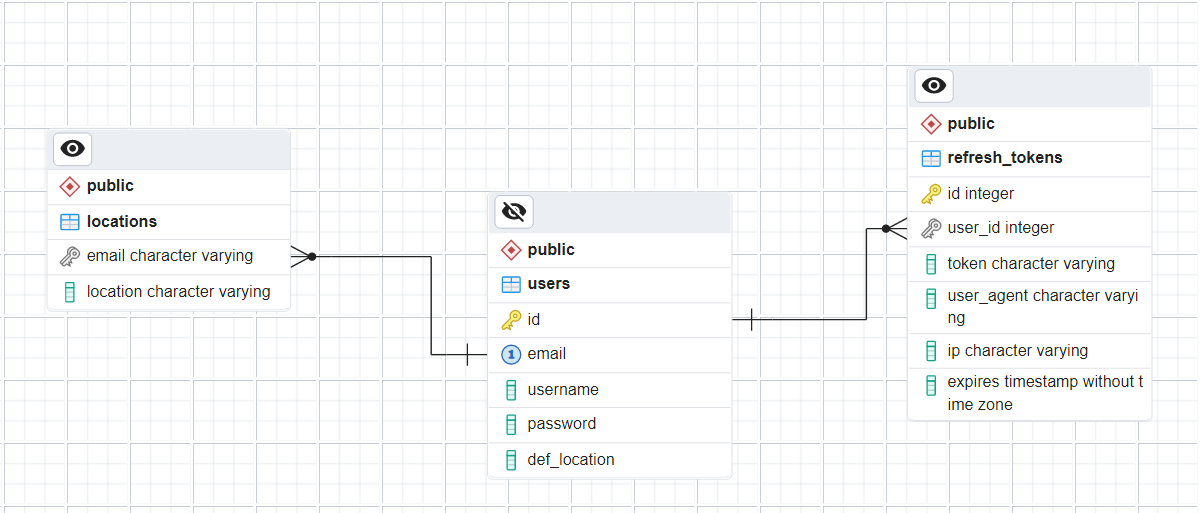
\includegraphics[width=\textwidth, height=0.3\textheight, keepaspectratio]{baza_podataka.png}
\caption{Shema baze podataka.}
\end{figure}

\subsection{Tablica Users}
Tablica \textit{users} sadrži informacije o registriranim korisnicima u našem sustavu. Svaki korisnik ima jedinstveni identifikator (ID), korisničko ime, lozinku i e-mail adresu koja je također jedinstvena.\begin{figure}[h]
\centering
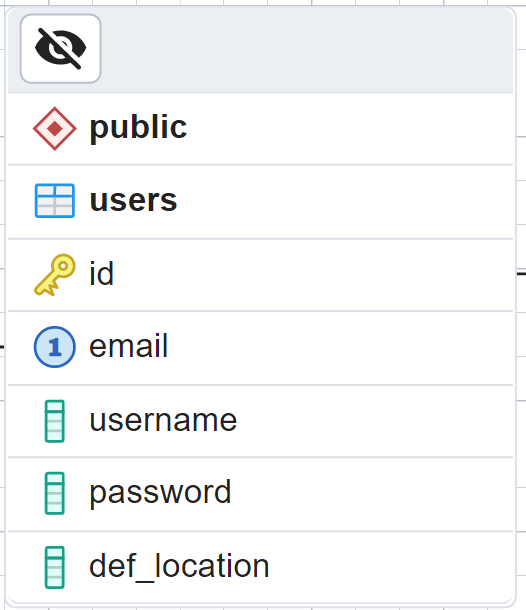
\includegraphics[width=\textwidth, height=0.3\textheight, keepaspectratio]{users.png}
\caption{Tablica \textit{users}.}
\end{figure}
\subsection{Tablica Locations}
Tablica \textit{locations} pohranjuje informacije o različitim lokacijama koje su korisnici unijeli kao svoje favorite. Sastoji se od e-maila i imena lokacije.
\begin{figure}
\centering
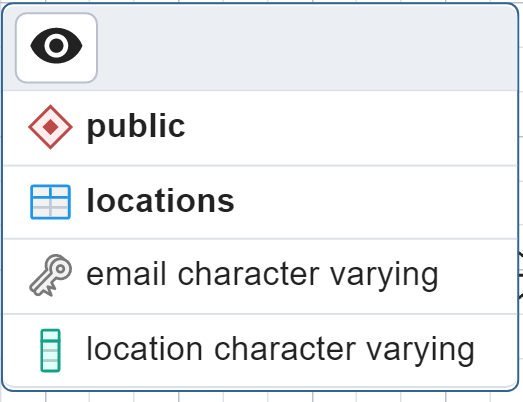
\includegraphics[width=\textwidth, height=0.2\textheight, keepaspectratio]{locations.png}
\caption{Tablica \textit{locations}.}
\end{figure}
\newpage
\subsection{Tablica Refresh Tokens}
Tablica \textit{refresh tokens} koristi se za pohranjivanje svih trenutno važećih osvježavajućih tokena za korisnike. Svaki zapis u tablici sadrži jedinstveni identifikator tokena, ID korisnika kojem token pripada, vrijeme isteka tokena, IP adresu i korisničkog posrednika \textit{(engl. User-Agent)}.
\newline

\begin{figure}[h]
\centering
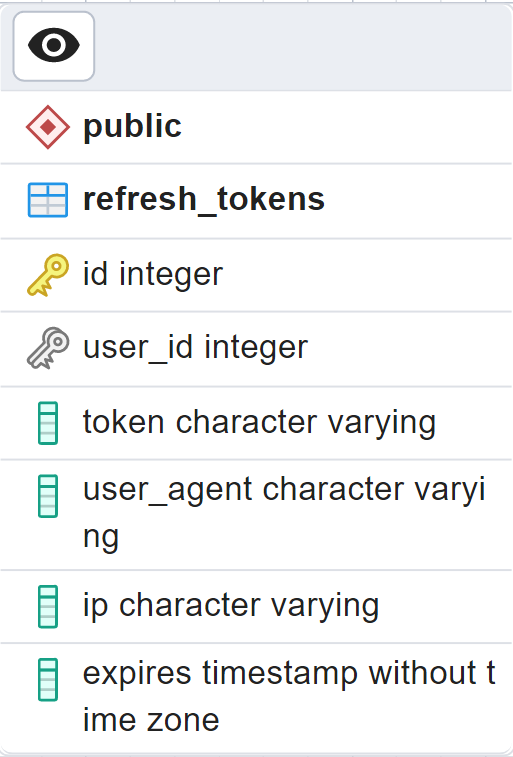
\includegraphics[width=\textwidth, height=0.3\textheight, keepaspectratio]{refresh_tokens.png}
\caption{Tablica \textit{refresh tokens}.}
\end{figure}

\newpage
\section{Testiranje i ispravljanje pogrešaka}

Testiranje i ispravljanje pogrešaka ključni su aspekti razvoja svake aplikacije. U ovom projektu koristili smo različite alate i pristupe kako bismo osigurali ispravnost našeg sustava.

\subsection{Postman}

Postman\cite{postman} je alat za razvoj API-ja koji programerima omogućuje da kreiraju, dijele i  testiraju API-je pružajući mogućnost organizacije zahtjeva, upravljanja okruženjima i analizu odgovora na zahtjeve. Postao je neizostavan dio svakodnevnog rada mnogih programera i tvrtki diljem svijeta. Moguće je izraditi različite vrste HTTP zahtjeva (GET, POST, PUT, DELETE itd.) te možemo priložiti potrebne parametre za svaki zahtjev, kao što su URL, zaglavlja (headers), tijelo (body) i druge. Postman omogućuje stvaranje i upravljanje kolekcijama zahtjeva, koje mogu biti vrlo korisne za testiranje i dokumentaciju API-ja. Kolekcija uključuje različite API zahtjeve za pristup različitim funkcionalnostima poslužitelja. Svaki zahtjev može vratiti različite odgovore, ovisno o tome je li bio uspješan ili je došlo do pogreške. Postman nam omogućuje analizu odgovora, omogućujući nam pregled statusnog koda, vrijeme odziva, veličinu odgovora i druge relevantne informacije. Također podržava razne metode autentifikacije. Na primjer, za autentifikaciju pomoću Bearer tokena, mogli bismo jednostavno dodati zaglavlje "Authorization" s vrijednošću "Bearer {token}" u naš zahtjev. Upravo ta funkcionalnost korištena je prilikom testiranja autentifikacije korisnika s klijentske aplikacije. Jednostavnom modifikacijom unutar Postman-a generiran je HTTP zahtjev koji bi bilo znatno teže kreirati samostalno.

\subsection{VS Code i evidentiranje grešaka}

Za razvijanje koda i praćenje njegovog izvođenja koristili smo integrirano razvojno okruženje \textit{(engl. IDE - Integrated Development Environment)} Visual Studio Code \cite{vscode}. VS Code je visoko konfigurabilno okruženje koje podržava velik broj programskih jezika i alata te pruža korisne značajke poput naglašavanja sintakse, automatskog dovršavanja koda i dubinskog praćenja koda. Važan dio ispravljanja pogrešaka bilo je i praćenje komunikacije između različitih dijelova aplikacije. Sustav je konfiguriran da evidentira ključne informacije tijekom izvođenja. Evidencija se koristila za praćenje tijeka izvođenja, detektiranje i ispravljanje pogrešaka te za analizu performansi sustava. Korištenje ispisa zapisnika \textit{(engl. logs)} se pokazalo ključnim u razvoju zbog efikasne identifikacije problema.

\section{Buduće Nadogradnje}

\subsection{Napredno upravljanje sesijama}
Upravljanje sesijama je ključni dio sigurne i učinkovite web aplikacije. Trenutačno se sesije koriste za održavanje konteksta između korisničkih zahtjeva, ali postoje mogućnosti za poboljšanje. Prvi korak u naprednom upravljanju sesijama mogao bi biti uvođenje sofisticiranijih strategija za upravljanje vremenskim rokovima sesija. Na primjer, mogli bismo implementirati automatsko zatvaranje sesija nakon određenog razdoblja neaktivnosti, što bi smanjilo opterećenje na poslužitelju i poboljšalo sigurnost. Druga moguća poboljšanja uključuju poboljšanje metoda autentifikacije sesija. To može uključivati upotrebu višefaktorske autentifikacije, pružajući tako dodatni sloj sigurnosti. Također, mogli bismo razviti metode za detekciju i prevenciju sesijskog otimanja, metoda napada koja uključuje neautorizirano preuzimanje valjane sesije korisnika.

\subsection{Implementacija Microservices arhitekture}
Arhitektura mikroservisa postala je sve popularnija u posljednjim godinama zbog brojnih prednosti. Mikroservisi omogućuju razbijanje aplikacije na manje, neovisne komponente koje se mogu razvijati i održavati odvojeno. Ovo može rezultirati boljom organizacijom koda, lakšim otkrivanjem i ispravljanjem grešaka, i većom skalabilnošću.
Uvođenje mikroservisa zahtijeva pažljivo planiranje i koordinaciju. Svaki servis mora biti dobro definiran, s jasno definiranim sučeljima i odgovornostima. Komunikacija između servisa mora biti sigurna i pouzdana. Također, potrebna je implementacija odgovarajućih mehanizama za nadzor i upravljanje servisima.

\subsection{Dodatne Integracije}
Integracija s drugim servisima ili API-ima može značajno proširiti mogućnosti našeg poslužitelja. Na primjer, mogli bismo integrirati servise za geolokaciju kako bismo korisnicima pružili preciznije informacije o vremenu na njihovoj trenutačnoj lokaciji. Postoji mogućnost integracije aplikacije s drugim meteorološkim servisima s ciljem proširenja
informacija kojima korisnici imaju pristup. Druga moguća integracija uključuje društvene mreže. Korisnici bi mogli dijeliti informacije o vremenu na društvenim mrežama izravno iz aplikacije.

\subsection{Sigurnost}
Sigurnost je od ključne važnosti za svaku web aplikaciju. Stoga, uvijek trebamo težiti poboljšanju naših sigurnosnih mjera. Jedan od načina za poboljšanje sigurnosti je uvođenje dodatnih mjera zaštite protiv različitih vrsta napada. Na primjer, mogli bismo implementirati metode za otkrivanje i ublažavanje DDoS napada, koji mogu uzrokovati ozbiljne probleme poslužitelju. Također, mogli bismo poboljšati naše metode autentifikacije i autorizacije. To može uključivati uvođenje višefaktorske autentifikacije, naprednijeg upravljanja lozinkama i korištenje biometrijskih podataka za autentifikaciju. Na kraju, trebali bismo razmotriti poboljšanje enkripcije. To može uključivati uvođenje naprednijih metoda enkripcije ili korištenje više slojeva enkripcije za dodatnu sigurnost.

\chapter{WeatherAPI: Pouzdan izvor vremenskih podataka}

WeatherAPI je ugledna platforma koja omogućuje pristup trenutnim, prognoziranim i povijesnim vremenskim podacima, geografskim informacijama, astronomskim podacima i još mnogo toga. Iako smo već razmotrili tehničke aspekte korištenja WeatherAPI-a u našoj aplikaciji, ovdje ćemo se više usredotočiti na projekt WeatherAPI, njegove suradnike i kako se održava i podržava. WeatherAPI je nastao kao odgovor na potrebu za pouzdanim, ažuriranim i sveobuhvatnim vremenskim podacima. Iza ovog projekta stoji tim stručnjaka iz različitih disciplina, uključujući meteorologiju, računalne znanosti, geografiju i statistiku. Tim se posvećuje pružanju najpreciznijih vremenskih informacija, koristeći napredne algoritme i modeliranje kako bi analizirao i interpretirao velike količine podataka. Njihov rad je podržan i nadograđen kroz suradnje s različitim vladinim, akademskim i privatnim institucijama. WeatherAPI surađuje s brojnim vladinim meteorološkim agencijama širom svijeta kako bi prikupio trenutne i povijesne vremenske podatke. Također koriste podatke dobivene od satelita, radarskih stanica i meteoroloških postaja za poboljšanje kvalitete i preciznosti svojih usluga. WeatherAPI koristi i mnogobrojnu zajednicu korisnika i programera koji neprestano nadograđuju i poboljšavaju njihove usluge. Ova zajednica ne samo da koristi i testira WeatherAPI, već i aktivno sudjeluje u njegovom razvoju, pružajući povratne informacije, identificirajući probleme i predlažući nove značajke. Zajednica također pruža korisne resurse, uključujući primjere koda, upute
i dokumentaciju, što olakšava novim korisnicima početnak korištenja WeatherAPI-a. Uz ovu snažnu podršku, WeatherAPI je postao izuzetno pouzdan izvor informacija o vremenskoj prognozi koji koriste tisuće aplikacija, web stranica i organizacija širom svijeta. Mi smo samo jedni od mnogih koji koriste WeatherAPI za pružanje točnih i ažuriranih vremenskih podataka našim korisnicima.

\chapter{Izrada neuronske mreže za predviđanje vremenskih uvjeta}

\section{Prikupljanje i Priprema Podataka}
Prvi korak u izgradnji svakog modela strojnog učenja je prikupljanje i priprema podataka. U našem slučaju, koristili bismo radarske snimke i povijesne vremenske podatke kao izvor podataka. Radarske snimke pružaju vizualni prikaz atmosferskih uvjeta dok povijesni vremenski podaci pružaju numeričke vrijednosti za različite parametre, poput temperature, vlažnosti zraka, tlaka zraka, brzine vjetra. Prikupljeni podatci trebali bi biti očišćeni i normalizirani. Čišćenje podataka uključuje uklanjanje nepostojećih ili neispravnih vrijednosti, dok normalizacija osigurava da svi podaci imaju slične raspone vrijednosti, što olakšava učenje neuronske mreže.

\section{Dizajn Neuronske Mreže}
Nakon što su podaci pripremljeni, sljedeći korak je dizajn neuronske mreže. Odlučili bismo se za arhitekturu mreže koja najbolje odgovara našim potrebama. Za vremenske prognoze, korisno bi bilo koristiti ponavljajuću neuronsku mrežu (RNN) ili konvolucijsku neuronsku mrežu (CNN), budući da su te vrste mreža posebno učinkovite za analizu vremenskih serija i slika, respektivno.

\subsection{Ponavljajuća Neuronska Mreža }
Ponavljajuće neuronske mreže (engl. reccurent neural network, RNN) su klasa umjetnih neuronskih mreža gdje veze između čvorova formiraju usmjereni graf duž sekvencije što znači da konekcije između čvorova mogu stvoriti ciklus. Takav sustav omogućava da izlaz jednog čvora mijenja stanje drugog čvora i omogućava mreži da koristi svoju unutarnju memoriju za obradu sekvenci ulaznih podataka, što je ključno za razumijevanje dinamike vremenskih serija poput meteoroloških podataka. RNN-ovi posjeduju povratne veze u svojoj strukturi, rezultirajući cirkuliranjem informacija u mreži i utjecajem na procesiranje svake nove točke podataka. Navedena svojstva čine RNN-ove posebno učinkovitima za rad s podacima gdje kontekst i vremenska ovisnost imaju veliki utjecaj, kao što je slučaj s vremenskim prognozama. Ipak, RNN-ovi su skloni problemima s nestajućim i eksplodirajućim gradijentima tijekom učenja, što može otežati treniranje. Zbog toga su razvijene varijacije RNN-a, kao što su LSTM (Long Short-Term Memory) i GRU (Gated Recurrent Units) koje uspješno rješavaju ove probleme.

\subsection{Konvolucijska Neuronska Mreža}
Konvolucijske neuronske mreže (engl. convolution nerual network, CNN) su regularizirane verzije višeslojnih perceptrona. Višeslojni perceptroni su obično potpuno povezane mreže, tj. svaki neuron u jednom sloju povezan je sa svim neuronima u sljedećem sloju. "Potpuna povezanost" ovih mreža čini ih sklonima prenaučenosti podataka. Tipični načini regularizacije, ili sprečavanja prenaučenosti, uključuju: kažnjavanje parametara tijekom treniranja (poput degradacije težina) ili smanjivanje povezanosti (preskočene veze, ispuštanje, itd.) Razvoj robustnih skupova podataka također povećava vjerojatnost da će CNN-ovi naučiti općenite principe koji karakteriziraju određeni skup podataka, umjesto pristranosti slabije populiranog seta. CNN-ovi imaju drugačiji pristup regularizaciji: koriste hijerarhijski obrazac u podacima i sastavljaju obrasce sve veće složenosti koristeći manje i jednostavnije obrasce uklesane u njihovim filterima. To znači da CNN-ovi koriste hijerarhijsku strukturu podataka koje obrađuju. Umjesto da pokušavaju obraditi cijelu sliku ili ulaz odjednom, CNN-ovi je razbijaju na manje, jednostavnije značajke, koje su predstavljene filterima. Ti se filteri primjenjuju na različita područja ulaza kako bi se izvukle relevantne informacije. Kako mreža napreduje kroz slojeve, ove se značajke kombiniraju i sastavljaju u složenije obrasce, omogućujući mreži učenje sve apstraktnijih reprezentacija ulaza. Ovaj hijerarhijski pristup omogućuje CNN-ovima da učinkovito uče složene obrasce u podacima, minimizirajući rizik od prenaučenosti. Konvolucijske neuronske mreže pokazale su se posebno učinkovitima u obradi slika. U kontekstu prognoze vremena, CNN-ovi mogu koristiti slike s radarskih snimaka i naučiti važne značajke koje će biti korisne za predviđanje. CNN-ovi koriste konvolucijske slojeve da automatski i adaptivno uče prostorne hijerarhije značajki iz ulaznih podataka.

\section{Treniranje mreže}
Treniranje neuronske mreže uključuje korištenje algoritama kao što je propagacija unatrag za postupno podešavanje težina mreže kako bi se minimizirala pogreška između predviđenih i stvarnih vrijednosti. Kao funkciju gubitka mogli bismo koristiti kvadratnu pogrešku, koja je često korištena za probleme regresije. Tijekom procesa treniranja, također bi bilo važno pratiti metrike poput točnosti i gubitka na skupu za validaciju kako bismo se uvjerili da mreža nije prenaučena (previše se prilagodi na podatke za treniranje). Drugi mogući način treniranja naše neuronske mreže bio bi pomoću genetski inspiriranog algoritma.

\subsection{Algoritam propagacije unatrag}
Propagacija unatrag (engl. backpropagation) je metoda korištena za treniranje umjetnih neuronskih mreža. Koristi se za računanje gradijenta funkcije gubitka s obzirom na težine u mreži. Algoritam je sastavljen od dvije faze: faza unaprijed i faza unatrag. U fazi unaprijed, ulaz prolazi kroz mrežu kako bi se generirao izlaz, a u fazi unatrag, gradijenti se propagiraju unatrag kroz mrežu s ciljem ažuriranja težina.

\subsection{Genetski inspirirani algoritmi}
Genetski inspirirani algoritmi koriste biološke procese poput nasljeđivanja, mutacija, selekcije i križanja za optimizaciju problema. Genetski algoritam, koji koristi set potencijalnih rješenja (nazvan populacija), a zatim kroz procese selekcije, križanja i mutacije nastoji pronaći najbolje rješenje. Genetski algoritmi mogu se koristiti za optimizaciju hiperparametara u neuronskim mrežama, uključujući broj skrivenih slojeva, broj neurona u svakom sloju, stopu učenja, i druge. Navedeno ima potencijal značajno unaprijediti performanse neuronske mreže, s obzirom da su hiperparametri vrlo utjecajni na njenu učinkovitost. Slično, algoritam roja čestica (engl. Particle Swarm Optimization, PSO) je još jedan genetski inspiriran algoritam koji se može koristiti za optimizaciju hiperparametara. PSO se temelji na konceptu roja čestica koji se kreću kroz prostor rješenja, gdje svaka čestica predstavlja potencijalno rješenje. Kretanje čestica je vođeno njihovom osobnom najboljom pozicijom i globalno najboljom pozicijom u prostoru rješenja.

\subsection{Primjena genetski inspiriranog algoritma}
Korištenje prethodno navedenih genetskih algoritama poput PSO bilo bi sastavljeno od sljedećih koraka:
\begin{itemize}
    \item Inicijalizacija: generiramo početnu populaciju potencijalnih rješenja. Svako rješenje predstavlja set hiperparametara mreže.
    \item Evaluacija: Izračunamo funkciju gubitka mreže za svako rješenje u populaciji.
    \item Selekcija: Odaberemo najbolja rješenja na temelju njihove funkcije gubitka.
    \item Križanje i Mutacija: Kombiniramo najbolja rješenja da bismo generirali novu populaciju i dodajemo male nasumične mutacije u hiperparametre da bismo održali raznolikost populacije.
    \item Iteracija: Ponavljamo korake 2-4 dok ne postignemo zadovoljavajući rezultat ili dok ne dostignemo maksimalan broj iteracija.
\end{itemize}
Primjena ovih algoritama mogla bi značajno poboljšati performanse neuronske mreže, omogućujući nam da efikasnije predviđamo vremenske uvjete.

\subsection{Evaluacija i podešavanje modela}
Nakon što je neuronska mreža trenirana, trebali bismo je evaluirati na testnom skupu podataka kako bismo dobili realnu ocjenu njezinih performansi. U slučaju da rezultati nisu zadovoljavajući, mijenjamo parametre mreže (kao što su broj slojeva, broj neurona, stopa učenja i tako dalje) kako bismo poboljšali performanse.

\subsection{Implementacija modela u poslužiteljskoj aplikaciji}
Konačno, nakon što smo zadovoljni performansama naše neuronske mreže, mogli bismo je integrirati u naš poslužitelj. To bi uključilo korištenje modela za predviđanje vremenskih uvjeta na temelju aktualnih i povijesnih podataka te pružanje tih predviđanja korisnicima naše aplikacije. Iako nismo mogli izvesti ovaj dio projekta zbog ograničenja pristupa podacima, vjerujemo da bi implementacija neuronske mreže za predviđanje vremenskih uvjeta značajno poboljšala funkcionalnost i korisnost naše aplikacije. Nadamo se da će budući razvoj i dostupnost podataka omogućiti ovakve poboljšanja.

\chapter{Teorija Kaosa}
Teorija kaosa je interdisciplinarna teorija koja prepoznaje osjetljivost početnih uvjeta u dinamičkim sustavima. Postala je popularna u pretkraj 20. stoljeća kroz radove znanstvenika kao što su Edward Lorenz. Teorija kaosa proučava kako male varijacije u početnim uvjetima mogu dovesti do dramatično različitih ishoda, poznatog kao "efekt leptira". U kontekstu meteorologije, atmosferski uvjeti su primjer kaotičnog sustava. Promjene u početnim uvjetima atmosferskih uvjeta, poput minimalnih promjena temperature ili vlažnosti zraka, mogu značajno utjecati na dugoročne vremenske uvjete. Osjetljivost na početne uvjete je ključna karakteristika kaotičnih sustava i predstavlja osnovni izazov u vremenskoj prognozi. Unatoč ovim izazovima, statističke metode i računalni modeli omogućuju izradu vremenskih prognoza. Ensembleska prognoza, metoda koja se široko koristi u meteorologiji, generira više mogućih ishoda na temelju malih varijacija početnih uvjeta. Kombinirajući ove ishode, moguće je stvoriti statističku prognozu koja pruža procjene vjerojatnosti za različite vremenske uvjete. Suvremeni računalni modeli koriste zakone fluidne dinamike, termodinamike i drugih područja fizike kako bi simulirali kretanje i interakciju atmosferskih plinova. Na temelju ovih simulacija i početnih uvjeta, moguće je stvoriti detaljne prognoze o vremenskim uvjetima. Međutim, zbog inherentne kaotične prirode atmosferskih sustava, dugoročne prognoze su manje precizne i često se izražavaju kao vjerojatnost. Pored toga, sve veća dostupnost podataka o atmosferi, uz sve veće računalne sposobnosti, omogućuje sve preciznije simulacije atmosferskih procesa. Također, integracija različitih izvora podataka, poput satelitskih snimaka, podataka sa zemaljskih stanica i podataka iz oceana, pomaže u poboljšanju početnih uvjeta za vremenske modele, doprinoseći preciznosti prognoza. U zaključku, teorija kaosa igra ključnu ulogu u razumijevanju i predviđanju vremenskih uvjeta. Unatoč izazovima koje predstavlja, primjena suvremenih statističkih metoda i naprednih računalnih modela omogućuje meteorolozima da stvaraju korisne i relativno točne vremenske prognoze. Ipak, zbog inherentne kaotične prirode vremenskih sustava, dugoročne prognoze uvijek će biti približne i predstavljene u obliku vjerojatnosti.

\chapter{Zaključak}
Razvoj web aplikacije za pronalaženje vremenskih uvjeta zahtijevao je uspješnu integraciju više tehnologija uključujući Flask, PostgreSQL, korisnički autentifikacijski sustav i sustav komunikacije s WeatherAPI-jem. Fokusiranje na jasnu strukturu koda i upotrebu modernih alata i praksi omogućio je razvoj čistog, efikasnog i sigurnog sustava. Kroz proces izgradnje aplikacije, posebno je naglašen značaj testiranja i ispravljanja pogrešaka. Korištenje aplikacije Postman bilo je instrumentalno za testiranje komunikacije između klijenta i poslužitelja, kao i između poslužitelja i API-ja. Isto tako, korištenje praćenja komunikacije iz razvojnog okruženja VS Code omogućilo je efikasno praćenje i rješavanje potencijalnih problema u radu aplikacije. Projekt je pokazao kako se kombiniranjem različitih tehnologija i pristupa može stvoriti snažna i funkcionalna web aplikacija. Kroz daljnje poboljšavanje i dodavanje novih značajki, aplikacija ima potencijal da postane još korisniji alat za pružanje preciznih vremenskih prognoza.

\printbibliography[title=Literatura]
\addcontentsline{toc}{chapter}{Literatura}


\begin{sazetak}
U okviru završnog rada je razvijen sustav za praćenje vremenske prognoze. Korišteni su Python i React Typescript, uz PostgreSQL bazu podataka. Implementirano je korisničko sučelje koje omogućuje interaktivan prikaz vremenskih podataka. Testiranje je provedeno korištenjem alata poput Postmana, logova i Visual Studio Code. Ostvarena je uspješna funkcionalnost sustava, što naglašava važnost korištenja različitih tehnologija i testiranja u razvoju web aplikacija.

\kljucnerijeci{vremenska prognoza, Python, React Typescript, PostgreSQL, korisničko sučelje, testiranje, Postman, web aplikacije}
\end{sazetak}

\engtitle{Weather forecast monitoring system}
\begin{abstract}
As part of the final project, a weather forecast monitoring system has been developed. Python and React Typescript were used, along with PostgreSQL as the database. A user interface has been implemented to provide an interactive display of weather data. Testing was performed using tools such as Postman, logs, and Visual Studio Code. The system has achieved successful functionality, highlighting the importance of utilizing different technologies and testing in web application development.

\keywords{weather forecast, Python, React Typescript, PostgreSQL, user interface, testing, Postman, web applications}
\end{abstract}

\end{document}
